\renewcommand*{\arraystretch}{1.1}

\subsection*{Interactive / update / 4}
\label{section:interactive-update-04}

\noindent\begin{tabularx}{\queryCardWidth}{|>{\queryPropertyCell}p{\queryPropertyCellWidth}|X|}
	\hline
	query & Interactive / update / 4 \\ \hline
%
	title & Add Forum
 \\ \hline
%
	pattern & \hfill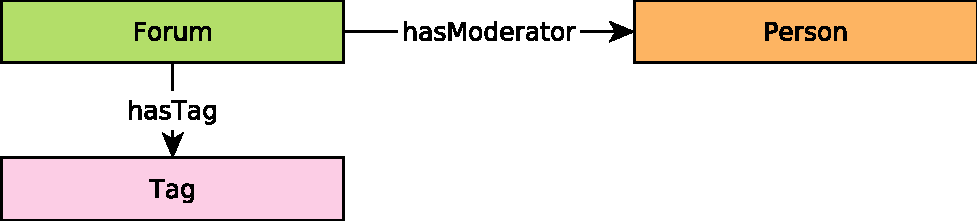
\includegraphics[scale=\patternscale,margin=0cm .2cm]{patterns/interactive-update-04}\hfill\vadjust{} \\ \hline
%
	desc. & Add a Forum to the social network.
 \\ \hline
%
	
		params &
		\innerCardVSpace{\begin{tabularx}{\attributeCardWidth}{|>{\paramNumberCell}c|>{\varNameCell}M|>{\typeCell}m{\typeWidth}|Y|} \hline
		$\mathsf{1}$ & Forum.id
 & ID
 &  \\ \hline
		$\mathsf{2}$ & Forum.title
 & String
 &  \\ \hline
		$\mathsf{3}$ & Forum.creationDate
 & DateTime
 &  \\ \hline
		$\mathsf{4}$ & Forum-hasModerator-\textgreater{}Person.id
 & ID
 &  \\ \hline
		$\mathsf{5}$ & Forum-hasTag-\textgreater{}Tag.id
 & \{ID\}
 &  \\ \hline
		\end{tabularx}}\innerCardVSpace \\ \hline
	
%
	
%
	%
	%
	%
	%
\end{tabularx}
\queryCardVSpace